\section{Results}
\label{sec:results}
\subsection{A compact prediction--storage trade-off}
External state improves shifted prediction MSE by 19.28\% with 28,848 mutable
bytes. Prediction-path tuning reaches 21.85\% with 1,932,488 bytes under the
evaluated Adam configuration. The difference in gain is 2.57 percentage
points; the difference in mutable storage is about 67-fold.
Figure~\ref{fig:tradeoff} and Table~\ref{tab:main} place this result beside the
other evaluated configurations. The external-state point is non-dominated
among these five configurations: no other point has both less mutable storage
and greater mean prediction gain.

\begin{figure}[tbp]
\centering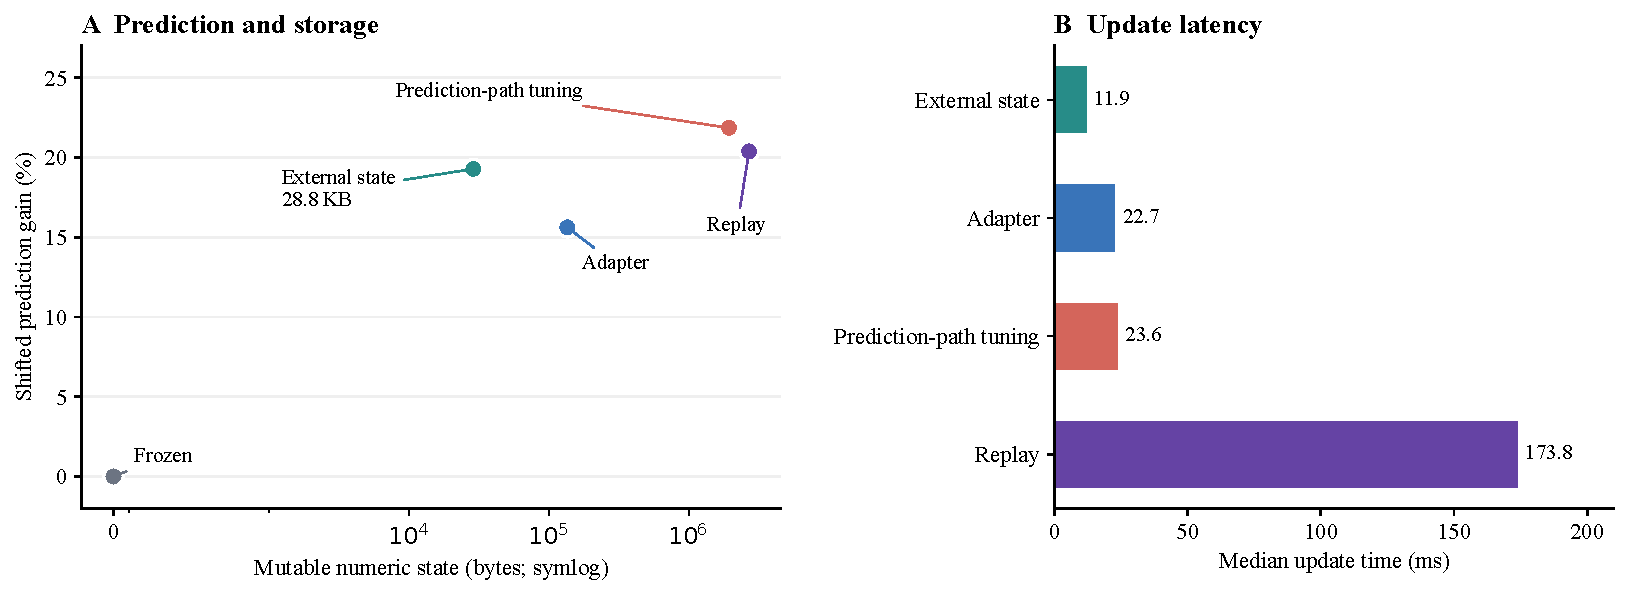
\includegraphics[width=\linewidth]{fig3_tradeoff.pdf}
\caption{\textbf{External state provides a compact deployment configuration.}
Left: prediction gain against peak mutable numeric storage for the five main
arms. Labels identify every point; the horizontal axis uses a symmetric-log
scale to include frozen prediction at zero bytes. Right: median update latency
for the adaptive arms. All arms use the same three-foundation, three-action-seed
design. These are configuration-specific memory and latency measurements.}
\label{fig:tradeoff}
\end{figure}
\begin{table}[tbp]
\centering\small
\caption{Main six-stage replay comparison. Gains use 126 shifted transitions per run after routing prefixes; all trainable arms use Adam. Mutable state excludes frozen weights and transient activations.}
\label{tab:main}
\begin{tabular}{@{}lrrrr@{}}
\toprule
Method & Pred. gain (\%) & Tracking (\%) & Bytes & Update (ms) \\
\midrule
Frozen & 0.00 & 0.00 & 0 & -- \\
External state & 19.28 & 3.80 & 28,848 & 11.90 \\
Adapter (Adam) & 15.61 & 3.47 & 135,232 & 22.72 \\
Prediction-path tuning (Adam) & 21.85 & 2.91 & 1,932,488 & 23.62 \\
Replay (Adam) & 20.38 & 3.35 & 2,693,128 & 173.83 \\
\bottomrule
\end{tabular}
\end{table}


The external-state mean prediction gain has a foundation-bootstrap 95\% CI
of 15.71\%--21.80\%. Its mean tracking gain is 3.80\%, and calibrated-source
return produces zero command correction. Median update time is 11.9 ms,
approximately half that of the adapter and prediction-path tuning arms.
External state thus improves prediction with a small allocation and a short
update time in this comparison. Appendix~\ref{app:extended} reports the
values for each foundation.

In the separate matched actuator-identification replay, external state obtains
19.72\% prediction gain and the routed matrix RLS obtains 0.58\%. That
comparison isolates actuator-space identification on the six-stage layout.
In the separate development protocol in Appendix~\ref{app:additional}, direct
output-space calibrators achieve larger prediction gains with less state.
Where the correction is applied therefore matters to this comparison.

\subsection{Prediction and action gains come from different components}
Table~\ref{tab:roles} makes the role of the residual matrices explicit.
Relative to scores alone, matrices add 9.22 percentage points of prediction
gain under shear and 25.12 points under attenuation. Yet the full and
score-only variants execute exactly the same commands in the paired
intervention. Removing the inverse makes action improvement zero.
The matrices improve predictions; the scores and inverse change commands.
The interventions separate these two effects of online adaptation.
\begin{table}[tbp]
\centering\small
\caption{Component intervention. Full and score-only commands are bitwise equal; matrix contribution is their difference in prediction gain.}
\label{tab:roles}
\begin{tabular}{@{}lrrrr@{}}
\toprule
Shift & Full gain (\%) & Scores (\%) & Matrix (points) & Tracking (\%) \\
\midrule
Shear & 8.13 & -1.09 & 9.22 & 43.99 \\
Attenuation & 32.63 & 7.51 & 25.12 & 3.88 \\
\bottomrule
\end{tabular}
\end{table}


The bounded-memory implementation preserves this behavior. Across the
36 traces in nine matched four-controller scenarios, the original and bounded
versions agree in observable
fields, and the first changed command occurs at decision five. This verifies
that the small runtime footprint does not depend on retaining an expanding
transition history. Throughout the main deployment runs, parameter hashes
and fixed-input semantic-logit hashes remain unchanged.

\subsection{The action correction improves closed-loop reward}
In registered attenuation, external state raises mean cumulative reward from
414.68 to 422.58. The paired reward improvement is 7.90, with a 95\% CI from
2.48 to 14.06. Figure~\ref{fig:control} shows how the reward difference
develops after the observation prefix; Table~\ref{tab:control} includes all
closed-loop comparison arms. The reward gain is positive on each of the three
tasks and across all five model seeds. These results show that the score-and-inverse path improves behavior in this
attenuation study, alongside the matrices' separate effect on prediction.

\begin{figure}[tbp]
\centering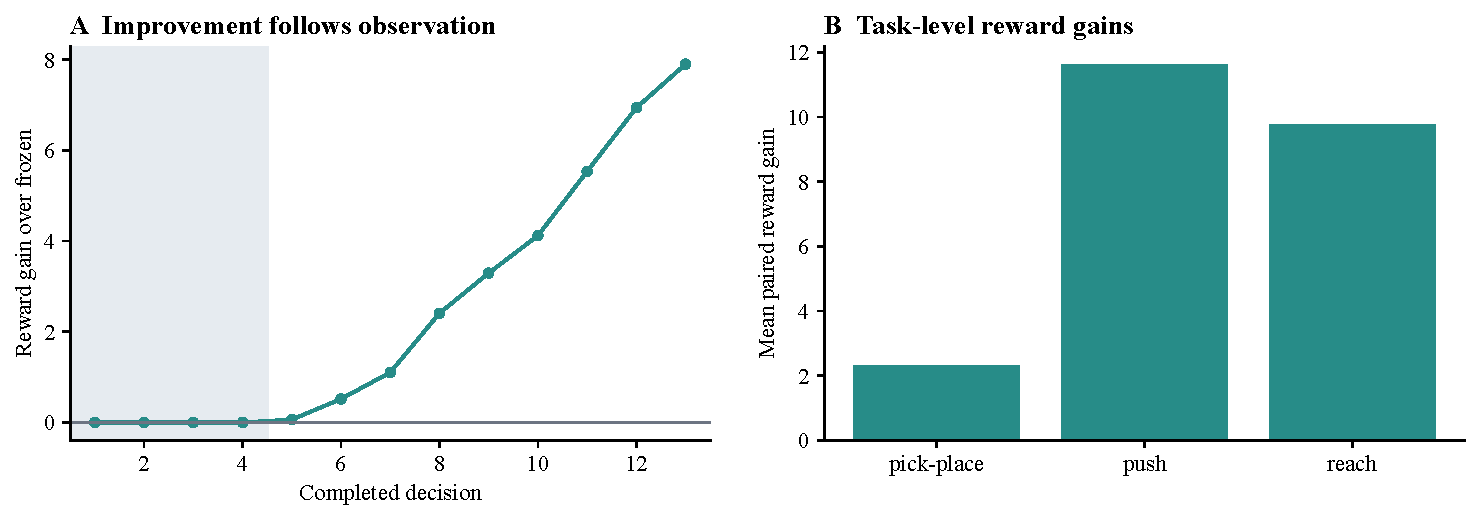
\includegraphics[width=0.95\linewidth]{fig4_control.pdf}
\caption{\textbf{Behavior changes after evidence is available.}
Left: mean cumulative reward difference between external state and frozen
control, plotted at completed decisions. The shaded prefix contains the first
four decisions; decision five is the earliest corrected command. Right: paired
reward gains by task. The separate attenuation study uses 75 trajectories per
arm. Reward is used for evaluation, not for updating external state.}
\label{fig:control}
\end{figure}
\begin{table}[tbp]
\centering\small
\caption{Closed-loop attenuation: 75 trajectories per arm; adaptation carries across replicas within each model/task pair. Reward and success are evaluation-only. Controller definitions appear in Appendix~\ref{app:control}.}
\label{tab:control}
\begin{tabular}{@{}lrr@{}}
\toprule
Method & Mean reward & Success (\%) \\
\midrule
Frozen & 414.68 & 53.33 \\
Prediction-model tuning (AdamW) & 422.19 & 66.67 \\
Oracle inverse (uncapped correction) & 485.50 & 80.00 \\
Gain-memory replay & 428.59 & 60.00 \\
Scalar RLS & 434.41 & 65.33 \\
External state & 422.58 & 66.67 \\
\bottomrule
\end{tabular}
\end{table}


\subsection{Shared predictive training supports several readouts}
Relative to the sequential checkpoint, joint training reduces action MSE by
17.10\% and normalized sensory prediction error by 0.75\%. Semantic accuracy
and image--text class retrieval rise by 1.80 and 1.81 percentage points,
respectively. These paired means use five action initializations
sharing a sensory foundation. Table~\ref{tab:joint} reports their intervals.
These changes show that joint updates improve both predictive and semantic
readouts relative to the sequential checkpoint. The complete three-stage comparison
in Appendix~\ref{app:joint} also shows the trade-off with action-only updates:
joint training improves class retrieval, while action-only updating achieves
the lower action error.
\begin{table}[tbp]
\centering\small
\caption{Joint training relative to the sequential checkpoint. Five action initializations share one sensory foundation. Intervals are paired 95\% bootstrap intervals.}
\label{tab:joint}
\begin{tabular}{@{}lrr@{}}
\toprule
Metric & Mean improvement & 95\% CI \\
\midrule
Action MSE reduction & 17.10\% & [14.04, 20.04]\% \\
Sensory MSE reduction & 0.75\% & [0.68, 0.83]\% \\
Semantic accuracy change & 1.80 points & [1.22, 2.44] points \\
Image--text retrieval change & 1.81 points & [0.19, 3.44] points \\
\bottomrule
\end{tabular}
\end{table}


The controlled probes in Appendix~\ref{app:probes} examine what the predictive
interface captures: ordered temporal structure, future observation statistics,
and image/audio factor associations. The training-stage pilot in
Appendix~\ref{app:bridge} then connects different trained checkpoints to the
same external-state interface. The probes test what the representation learns; the pilot tests how the
external correction behaves on checkpoints from different training stages.
